\documentclass[]{article}

% Options for packages loaded elsewhere
\PassOptionsToPackage{unicode}{hyperref}
\PassOptionsToPackage{hyphens}{url}
\PassOptionsToPackage{dvipsnames,svgnames,x11names}{xcolor}

\usepackage{xcolor}
\usepackage[margin=1in]{geometry}
\usepackage{amsmath,amssymb}
\setcounter{secnumdepth}{-\maxdimen} % remove section numbering
\usepackage{iftex}
\ifPDFTeX
  \usepackage[T1]{fontenc}
  \usepackage[utf8]{inputenc}
  \usepackage{textcomp} % provide euro and other symbols
\else % if luatex or xetex
  \usepackage{unicode-math} % this also loads fontspec
  \defaultfontfeatures{Scale=MatchLowercase}
  \defaultfontfeatures[\rmfamily]{Ligatures=TeX,Scale=1}
\fi
\usepackage{lmodern}

% Use upquote if available, for straight quotes in verbatim environments
\IfFileExists{upquote.sty}{\usepackage{upquote}}{}
\IfFileExists{microtype.sty}{%
  \usepackage[]{microtype}
  \UseMicrotypeSet[protrusion]{basicmath} % disable protrusion for tt fonts
}{}

\makeatletter
\@ifundefined{KOMAClassName}{%
  \IfFileExists{parskip.sty}{%
    \usepackage{parskip}
  }{% else
    \setlength{\parindent}{0pt}
    \setlength{\parskip}{6pt plus 2pt minus 1pt}}
}{% if KOMA class
  \KOMAoptions{parskip=half}}
\makeatother

\usepackage{graphicx}
\makeatletter
\newsavebox\pandoc@box
\newcommand*\pandocbounded[1]{%
  \sbox\pandoc@box{#1}%
  \Gscale@div\@tempa{\textheight}{\dimexpr\ht\pandoc@box+\dp\pandoc@box\relax}%
  \Gscale@div\@tempb{\linewidth}{\wd\pandoc@box}%
  \ifdim\@tempb\p@<\@tempa\p@\let\@tempa\@tempb\fi%
  \ifdim\@tempa\p@<\p@\scalebox{\@tempa}{\usebox\pandoc@box}%
  \else\usebox{\pandoc@box}%
  \fi%
}
\def\fps@figure{htbp}
\makeatother

\setlength{\emergencystretch}{3em}
\providecommand{\tightlist}{%
  \setlength{\itemsep}{0pt}\setlength{\parskip}{0pt}}
\usepackage{bookmark}
\IfFileExists{xurl.sty}{\usepackage{xurl}}{}
\urlstyle{same}

\hypersetup{
  pdftitle={ISTx1003 prosjekt: Tittel (gi projektet en informativ tittel)},
  pdfauthor={Gruppenummer},
  colorlinks=true,
  linkcolor={Maroon},
  filecolor={Maroon},
  citecolor={Blue},
  urlcolor={blue},
  pdfcreator={LaTeX via pandoc}}

\title{ISTx1003 prosjekt: Tittel (gi projektet en informativ tittel)}
\author{Gruppenummer}
\date{\today}

\begin{document}
\maketitle

Rapporten gir maks 50 poeng. Fordeling av poengene vises for hver del.
Hver del blir vurdert etter:
\begin{itemize}
\tightlist
\item faglig nivå
\item korrekthet
\item presentasjon og lesbarhet
\end{itemize}

% Inkluder kapitler
\subsection{Sammendrag/Abstract (max 500 ord) (10 poeng)}\label{sammendragabstract-max-500-ord-10-poeng}

Formålet med sammendraget er å gi en kort og presis oppsummering av
prosjektet deres. Det er en selvstendig tekst som plasseres før selve
rapporten begynner (men skriv den til slutt). Sammendraget bør inneholde
følgende deler:

\begin{enumerate}
\def\labelenumi{\arabic{enumi}.}
\tightlist
\item
  Start med å tydelig beskrive formålet med prosjektet. Hvilket problem
  forsøker dere å løse? Hvilket spørsmål ønsker dere å besvare? Beskriv
  forskningsspørsmålet/hypotesen. Det er viktig å være kortfattet og
  konkret.
\item
  Beskriv dataene dere brukte. Inkluder lenken til datasettet her.
  Hvilket datasett benyttet dere? Deklarer størrelse på datasettet
  (antal observasjoner, antal variabler), typer variabler og
  responsvariabel.
\item
  Beskriv metodene: Hvordan analyserte dere dataene? Hvilke verktøy,
  teknikker eller metoder brukte dere? Regresjon, klassifisering,
  klyngeanalyse? Vær spesifisk, men unngå for mange detaljer.
\item
  Oppsummer de viktigste funnene. I hoveddelen av sammendraget skal dere
  oppsummere de viktigste resultatene fra prosjektet og kort tolke dem
  (altså, hva betyr resultatene?). Fremhev de mest betydningsfulle
  funnene, og gi nok informasjon til at leseren får et inntrykk av hva
  dere har oppdaget.
\item
  (Valgfritt) Fremhev betydningen av resultatene. Forklar hvorfor
  og/eller hvordan funnene dine er viktige. Fremhev eventuelle nye eller
  uventede funn, og forklar hvordan de bidrar til økt forståelse av
  temaet.
\end{enumerate}

\subsection{Introduksjon (10 poeng)}\label{introduksjon-10-poeng}

\begin{itemize}
\item
  Gi en kort introduksjon til den overordnede problemstillingen eller
  oppgaven dere har valgt, samt datasettet dere bruker. Dette kan for
  eksempel være en klassifiseringsoppgave (f.eks. å forutsi om en
  pasient utvikler hjertesykdom eller ikke) eller en prediksjonsoppgave
  (f.eks. å forutsi prisen på en Airbnb). Definer tydelig avgrensningen
  for prosjektet deres. Hvilket spesifikt problem forsøker dere å løse?
\item
  Beskriv kilden til datasettet, og oppgi en referanse til hvor
  datasettet kommer fra.
\item
  Beskriv formålet med prosjektet mer detaljert. Hvilke konkrete
  spørsmål ønsker dere å besvare i prosjektet? Prøver dere å finne
  metoden som gir best resultater, eller en metode som gir gode
  resultater samtidig som den er enkel og effektiv å bruke? Hvem er
  målgruppen? Forsøker dere å undersøke sammenhenger mellom ulike
  variabler? Prøver dere å finne viktige prediktorer for
  klassifiseringen? Eller ønsker dere å oppnå en bedre og mer
  innsiktsfull forståelse av et bestemt tema eller fagområde?
\end{itemize}

\subsection{Beskrivende dataanalyse (5 poeng)}\label{beskrivende-dataanalyse-5-poeng}

Her bør du gjennomføre en kort deskriptiv dataanalyse for å få en
oversikt over datasettet. Det betyr at man lager noen visualiseringer
for å forstå dataene bedre, og at man beregner noen enkle ting. Fokuser
på det som er relevant for modelleringen, og bruk sunn fornuft. For mye
detaljer eller figurer uten forklaring og tydelige akseetiketter er ikke
nyttige for leseren.

Du kan for eksempel:

\begin{itemize}
\tightlist
\item
  Presentere deskriptiv statistikk, som gjennomsnitt, median,
  standardavvik og varians, for å beskrive datasettets sentraltendens,
  variasjon og fordeling.
\item
  Bruke spredningsdiagrammer (scatter plots) og korrelasjonsmatriser for
  å undersøke sammenhenger mellom ulike variabler.
\item
  Bruke histogrammer for å vise fordelingen til relevante variabler.
\item
  Bruke boksplott (box plots) for å undersøke fordeling, variasjon og
  eventuelle uteliggere.
\end{itemize}

Resultatene bør forklares i teksten, med særlig fokus på funn som kan
være relevante for den videre modelleringen. Skriv en kort legende under
hver grafikk, slik at det blir tydelig hva grafikken viser.

\subsection{Metoder (10 poeng)}\label{metoder-10-poeng}

% \begin{itemize}
% \item
%   Beskriv metodene dere bruker i prosjektet, og forklar i detalj hvordan
%   dere har anvendt dem. Dere bør bruke metoder fra mist 2 av de 3
%   temaene i kurset (regresjon, klassifikasjon, klyngeanalyse).
% \item
%   Forklar kort hvorfor metodene passer for datasett og problemstillingen
%   dere har valgt.
% \item
%   \textbf{Det er viktig at dere bare bruker metoder som er tilpasset
%   nivået i dette kurset -- bruk bare metoder dere lærer om her. Hold det
%   enkelt og realistisk, ikke bruk komplekse metoder som dere ikke
%   forstår, bare fordi KI foreslår det.}
% \item
%   Beskriv hvordan dere evaluerer metodene, hvis det er mulig. Evaluer
%   modellen(e) ved å bruke passende verktøy, for eksempel residualanalyse
%   eller vurdering av prediksjonsytelse (som sensitivitet og spesifisitet
%   i en binær klassifiseringsoppgave).
% \item
%   (Valgfritt) Diskuter mulige begrensninger ved metodene og de valgte
%   evalueringsmålene. Vurder for eksempel om et bestemt mål kan gi et
%   misvisende bilde av modellens ytelse, eller om det finnes egenskaper
%   ved datasettet som gjør en metode mindre egnede.
% \end{itemize}

I dette prosjektet kombinerer vi metoder fra to av hovedtemaene i kurset: \textbf{uovervåket klyngeanalyse} ($k$-Means, hierarkisk klyngeanalyse og PCA) og \textbf{veiledet klassifikasjon} ($K$-nærmeste naboer og logistisk regresjon). Denne kombinasjonen passer svært godt til problemstillingen vår: Først undersøker vi hvilke naturlige grupperinger som oppstår i de syv standardiserte lydvariablene ($Z$-verdier fra kapittel 3) uten at modellen kjenner til sjangrene, og deretter tester vi hvor mye bedre vi kan predikere de fem sjangerfamiliene når en klassifikasjonsmodell faktisk får lære sammenhengen mellom lydegenskaper og sjanger fra treningsdata.

\subsubsection{Tema 1: Uovervåket klyngeanalyse ($k$-Means, hierarkisk klyngeanalyse og PCA)}
For å finne naturlige grupperinger i lyddataene benytter vi \textbf{$k$-Means klyngeanalyse}. $k$-Means deler de $n = 2500$ sangene inn i $k$ disjunkte klynger $C_1, \dots, C_k$ ved å minimere den totale kvadrerte euklidske avstanden (Within-Cluster Sum of Squares, WCSS / Inertia) fra hver sang $z_i$ til klyngesenteret $\mu_c$ i klyngen den tilhører:
\[
\text{WCSS} = \sum_{c=1}^{k} \sum_{z_i \in C_c} \| z_i - \mu_c \|^2
\]
Algoritmen initialiserer $k$ klyngesentre og veksler iterativt mellom (1) å tilordne hver sang til det nærmeste klyngesenteret målt i euklidsk avstand, og (2) å oppdatere hvert klyngesenter som gjennomsnittsvektoren av sangene i klyngen, helt til konvergens.

For å velge antall klynger $k$ evaluerte vi $k \in \{2, \dots, 10\}$ ved hjelp av albue-metoden (WCSS) og gjennomsnittlig silhuett-score (figur~\ref{fig:elbow_silhouette}). Vi valgte $k = 5$ klynger, både fordi fallet i WCSS avtar merkbart rundt $k = 4\text{--}5$, og fordi $k = 5$ gir en direkte én-til-én-sammenligning med de fem overordnede sjangerfamiliene i datasettet.

\begin{figure}[htbp]
    \centering
    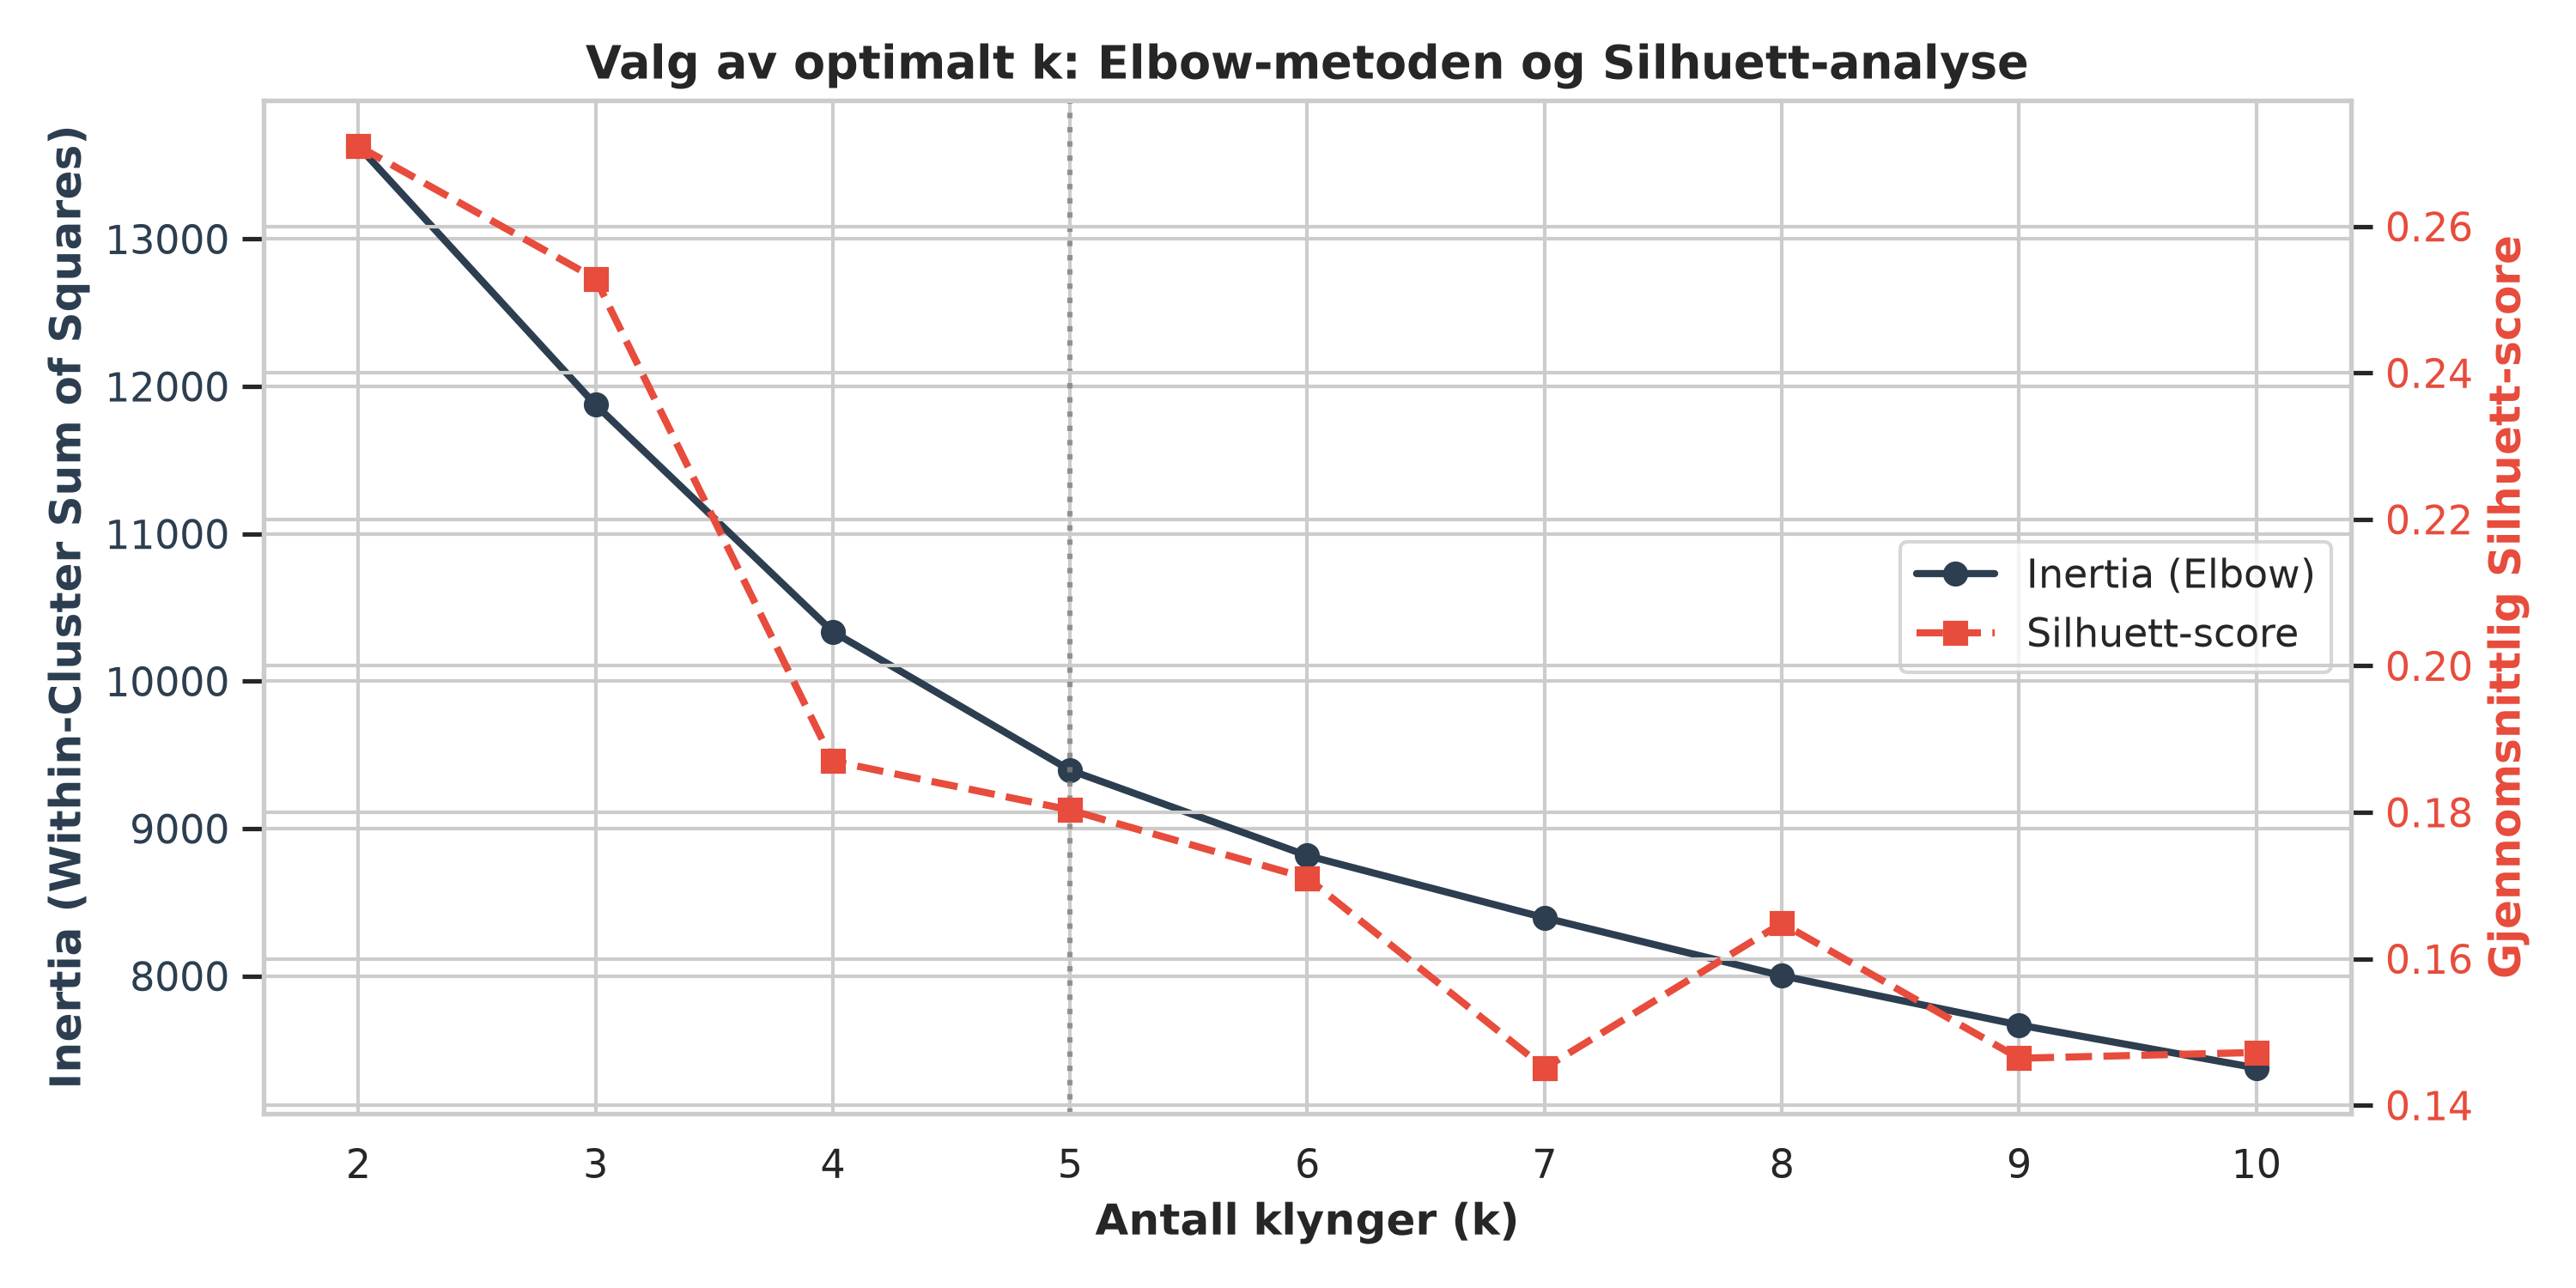
\includegraphics[width=0.88\linewidth]{figurer/1_elbow_and_silhouette.png}
    \caption{Valg av antall klynger $k$ for $k$-Means: WCSS / Inertia (albue-metoden, venstre akse) og gjennomsnittlig silhuett-score (høyre akse) for $k \in \{2, \dots, 10\}$. Den stiplede linjen markerer valgt $k = 5$.}
    \label{fig:elbow_silhouette}
\end{figure}

Som et supplement gjennomførte vi \textbf{agglomerativ hierarkisk klyngeanalyse} med \textbf{Wards kobling} på et tilfeldig utvalg på 100 sanger (figur~\ref{fig:dendrogram}). Algoritmen starter med hver sang som sin egen klynge nederst i et tre (dendrogram), og slår trinnvis sammen de to klyngene som gir minst økning i total innenfor-klynge-varians. Ved å kutte dendrogrammet horisontalt ved avstand $d = 10{,}5$ får vi fem hovedgrener, som lar oss kontrollere om en hierarkisk metode uten forhåndsbestemt $k$ støtter klyngestrukturen fra $k$-Means.

\begin{figure}[htbp]
    \centering
    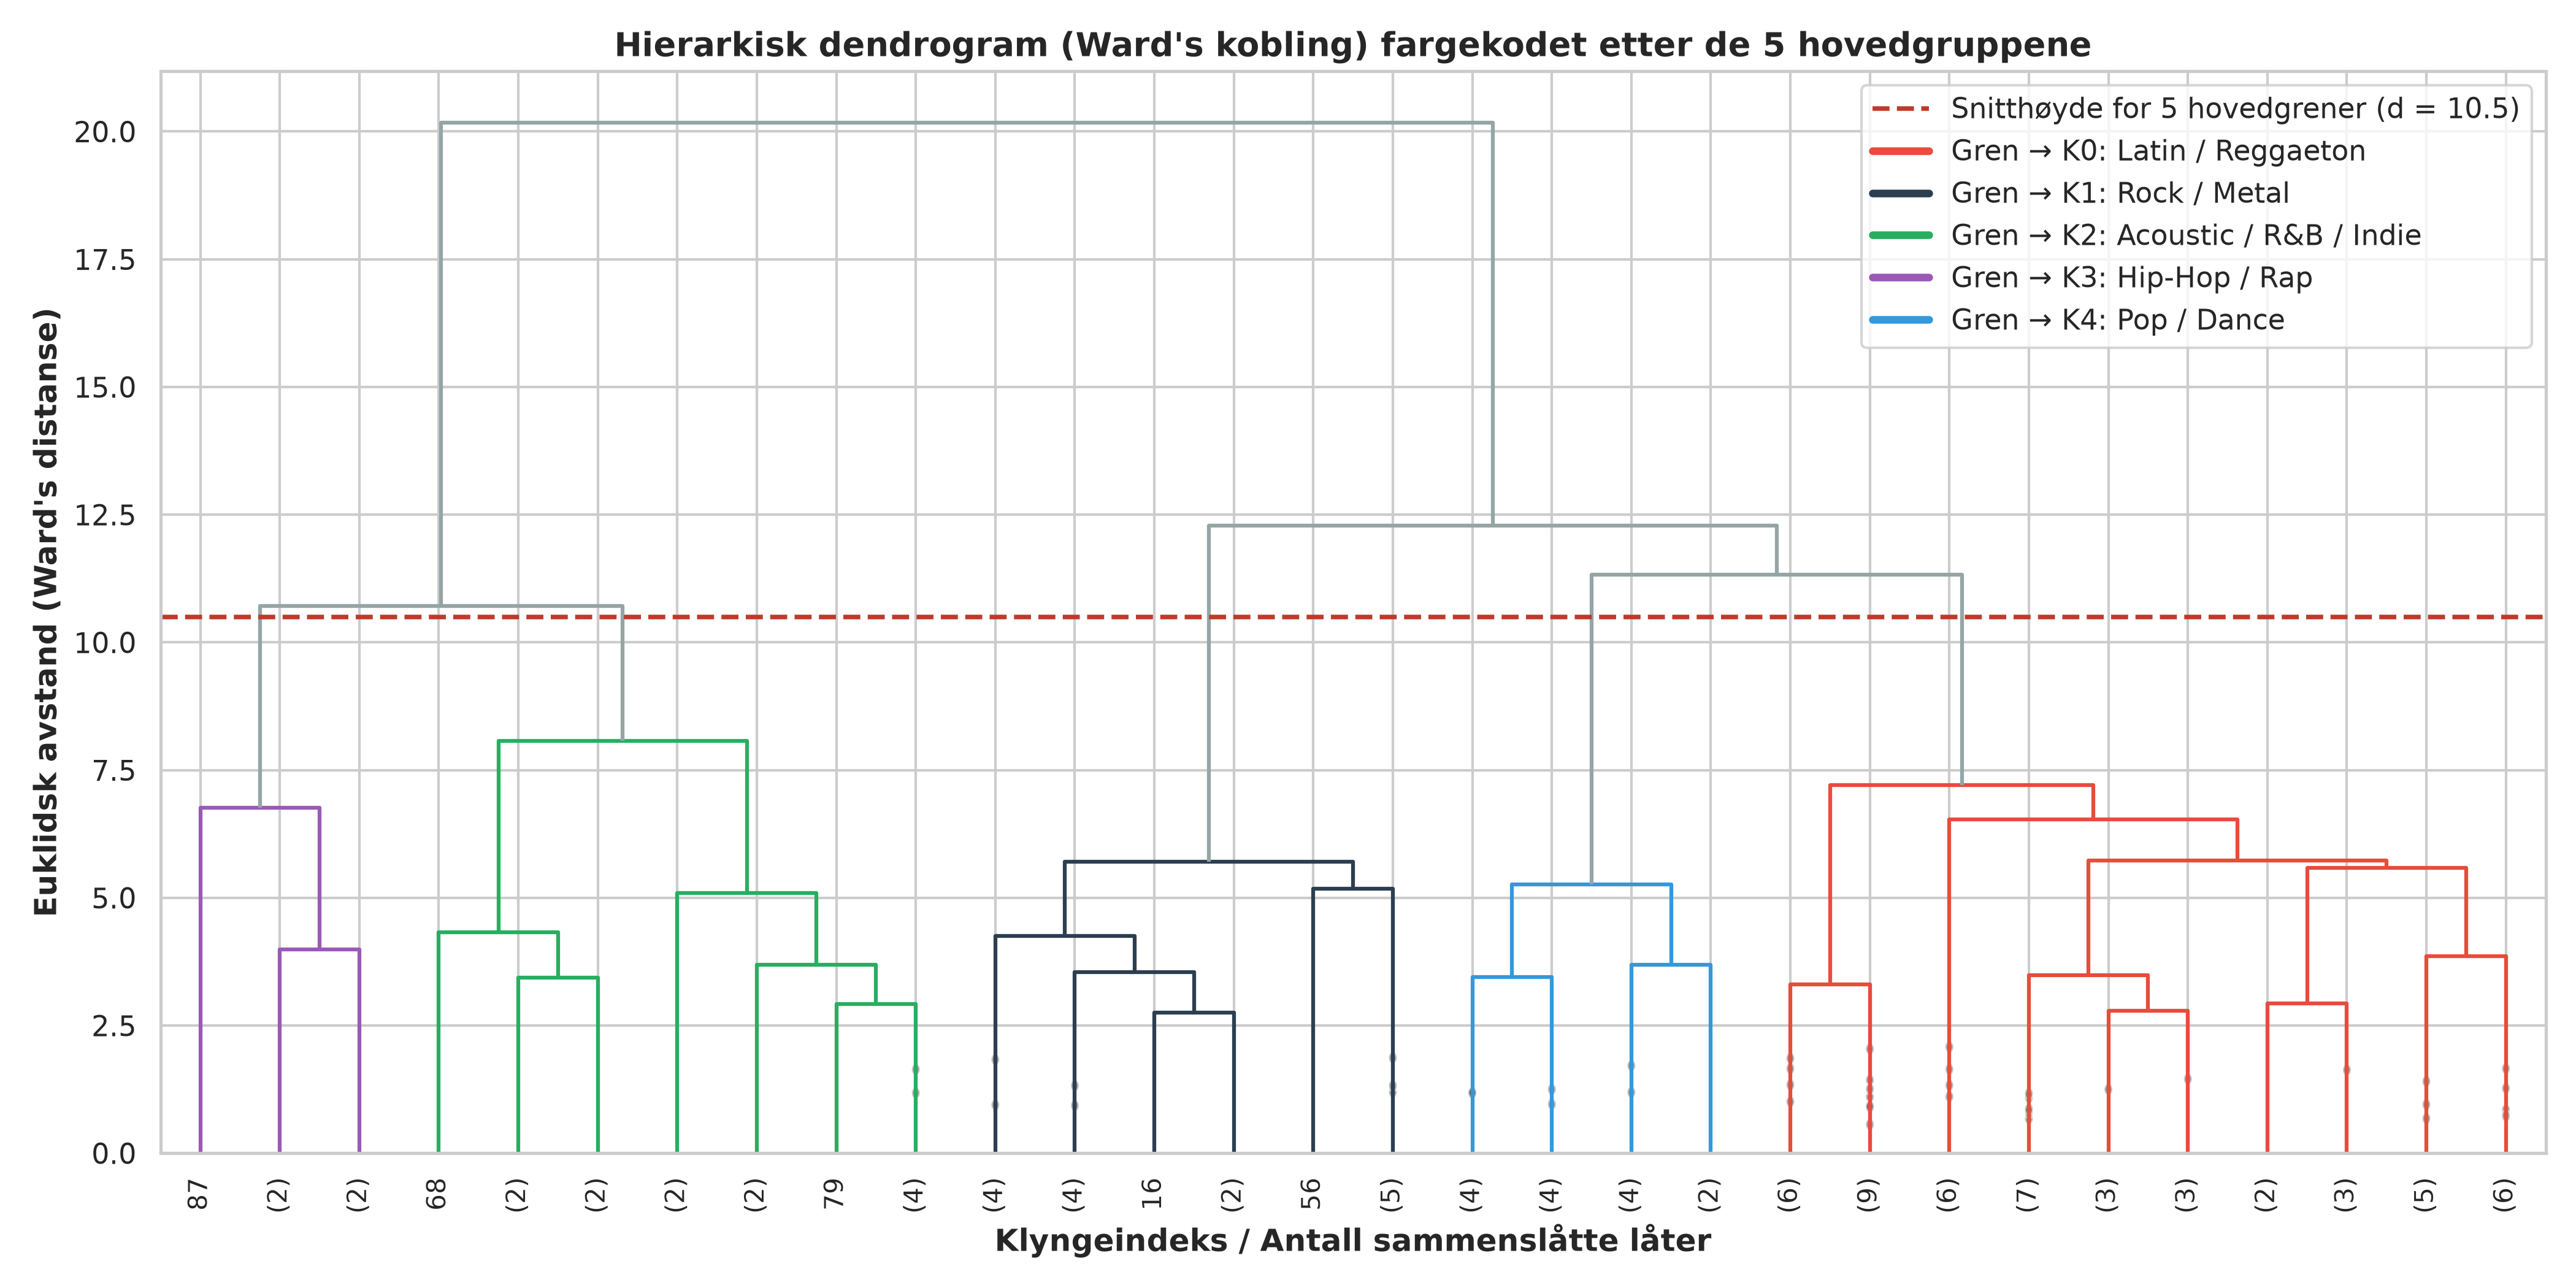
\includegraphics[width=0.95\linewidth]{figurer/4_hierarchical_dendrogram.png}
    \caption{Hierarkisk dendrogram med Wards kobling for et tilfeldig utvalg på 100 sanger. Den røde stiplede linjen ved avstand $d = 10{,}5$ markerer snitthøyden for 5 hovedgrener, fargekodet etter tilhørende $k$-Means-klynge.}
    \label{fig:dendrogram}
\end{figure}

Fordi klyngene befinner seg i et syvdimensjonalt rom, bruker vi \textbf{hovedkomponentanalyse (PCA)} for å visualisere klyngene i to dimensjoner. PCA konstruerer ortogonale lineærkombinasjoner av de syv variablene ($\text{PC1}$ og $\text{PC2}$, som til sammen forklarer $52{,}3\,\%$ av den totale variansen), slik at vi kan plotte både klynger og faktiske sjangre i samme todimensjonale koordinatsystem.

\subsubsection{Tema 2: Veiledet klassifikasjon ($K$-nærmeste naboer og logistisk regresjon)}
I prosjektets andre del formulerer vi sjangeridentifikasjon som en \textbf{veiledet klassifikasjonsoppgave} på de $n = 1566$ sangene som har kjent sjanger i datasettet. Her er de syv lydvariablene prediktorer $\mathbf{x}_i$, mens sjangerfamilien (\texttt{Genre\_Family} med 5 klasser) er den kategoriske responsvariabelen $y_i$. Vi deler disse sangene stratifisert inn i et \textbf{treningssett på $80\,\%$} ($1252$ sanger) og et uavhengig \textbf{testsett på $20\,\%$} ($314$ sanger), slik at sjangrenes relative fordeling er lik i begge sett. Standardiseringen ($Z$-score) tilpasses kun på treningssettet og brukes deretter til å transformere testsettet for å unngå datalekkasje.

Vi anvender og sammenligner to klassifikasjonsmetoder fra pensum:
\begin{enumerate}
\tightlist
\item
  \textbf{$K$-nærmeste naboer (KNN):} En ikke-parametrisk metode som klassifiserer en ny sang i testsettet ved å finne de $K$ sangene i treningssettet som ligger nærmest i euklidsk avstand i det syvdimensjonale lydrommet, og tilordne sangen til den sjangeren som har flertall blant disse $K$ naboene:
  \[
  \hat{P}(Y = j \mid X = \mathbf{x}_0) = \frac{1}{K} \sum_{i \in \mathcal{N}_0} I(y_i = j)
  \]
  Valget av hyperparameteren $K$ styrer avveiningen mellom skjevhet og varians (bias--variance tradeoff): lav $K$ gir en fleksibel grense med høy varians (fare for overtilpasning), mens høy $K$ gir jevnere beslutningsgrenser. Ved hjelp av 5-fold kryssvalidering på treningssettet for odde verdier $K \in \{1, 3, \dots, 35\}$ fant vi at $K = 15$ ga høyest kryssvalidert treffsikkerhet ($53{,}5\,\%$, figur~\ref{fig:knn_k}).
\item
  \textbf{Multinomial logistisk regresjon:} En parametrisk lineær klassifikasjonsmodell som estimerer sannsynligheten for hver av de $M = 5$ sjangerklassene ved hjelp av en lineær prediktor $\eta_{ik} = \beta_{0k} + \boldsymbol{\beta}_k^\top \mathbf{z}_i$ og softmax-funksjonen:
  \[
  P(Y_i = k \mid \mathbf{z}_i) = \frac{e^{\beta_{0k} + \boldsymbol{\beta}_k^\top \mathbf{z}_i}}{\sum_{m=1}^{M} e^{\beta_{0m} + \boldsymbol{\beta}_m^\top \mathbf{z}_i}}
  \]
  Ved å sammenligne logistisk regresjon (lineære klassegrenser) med KNN (ikke-lineære, lokale klassegrenser) får vi undersøkt om sjangergrensene i lydrommet er lineære eller mer sammensatte.
\end{enumerate}

\begin{figure}[htbp]
    \centering
    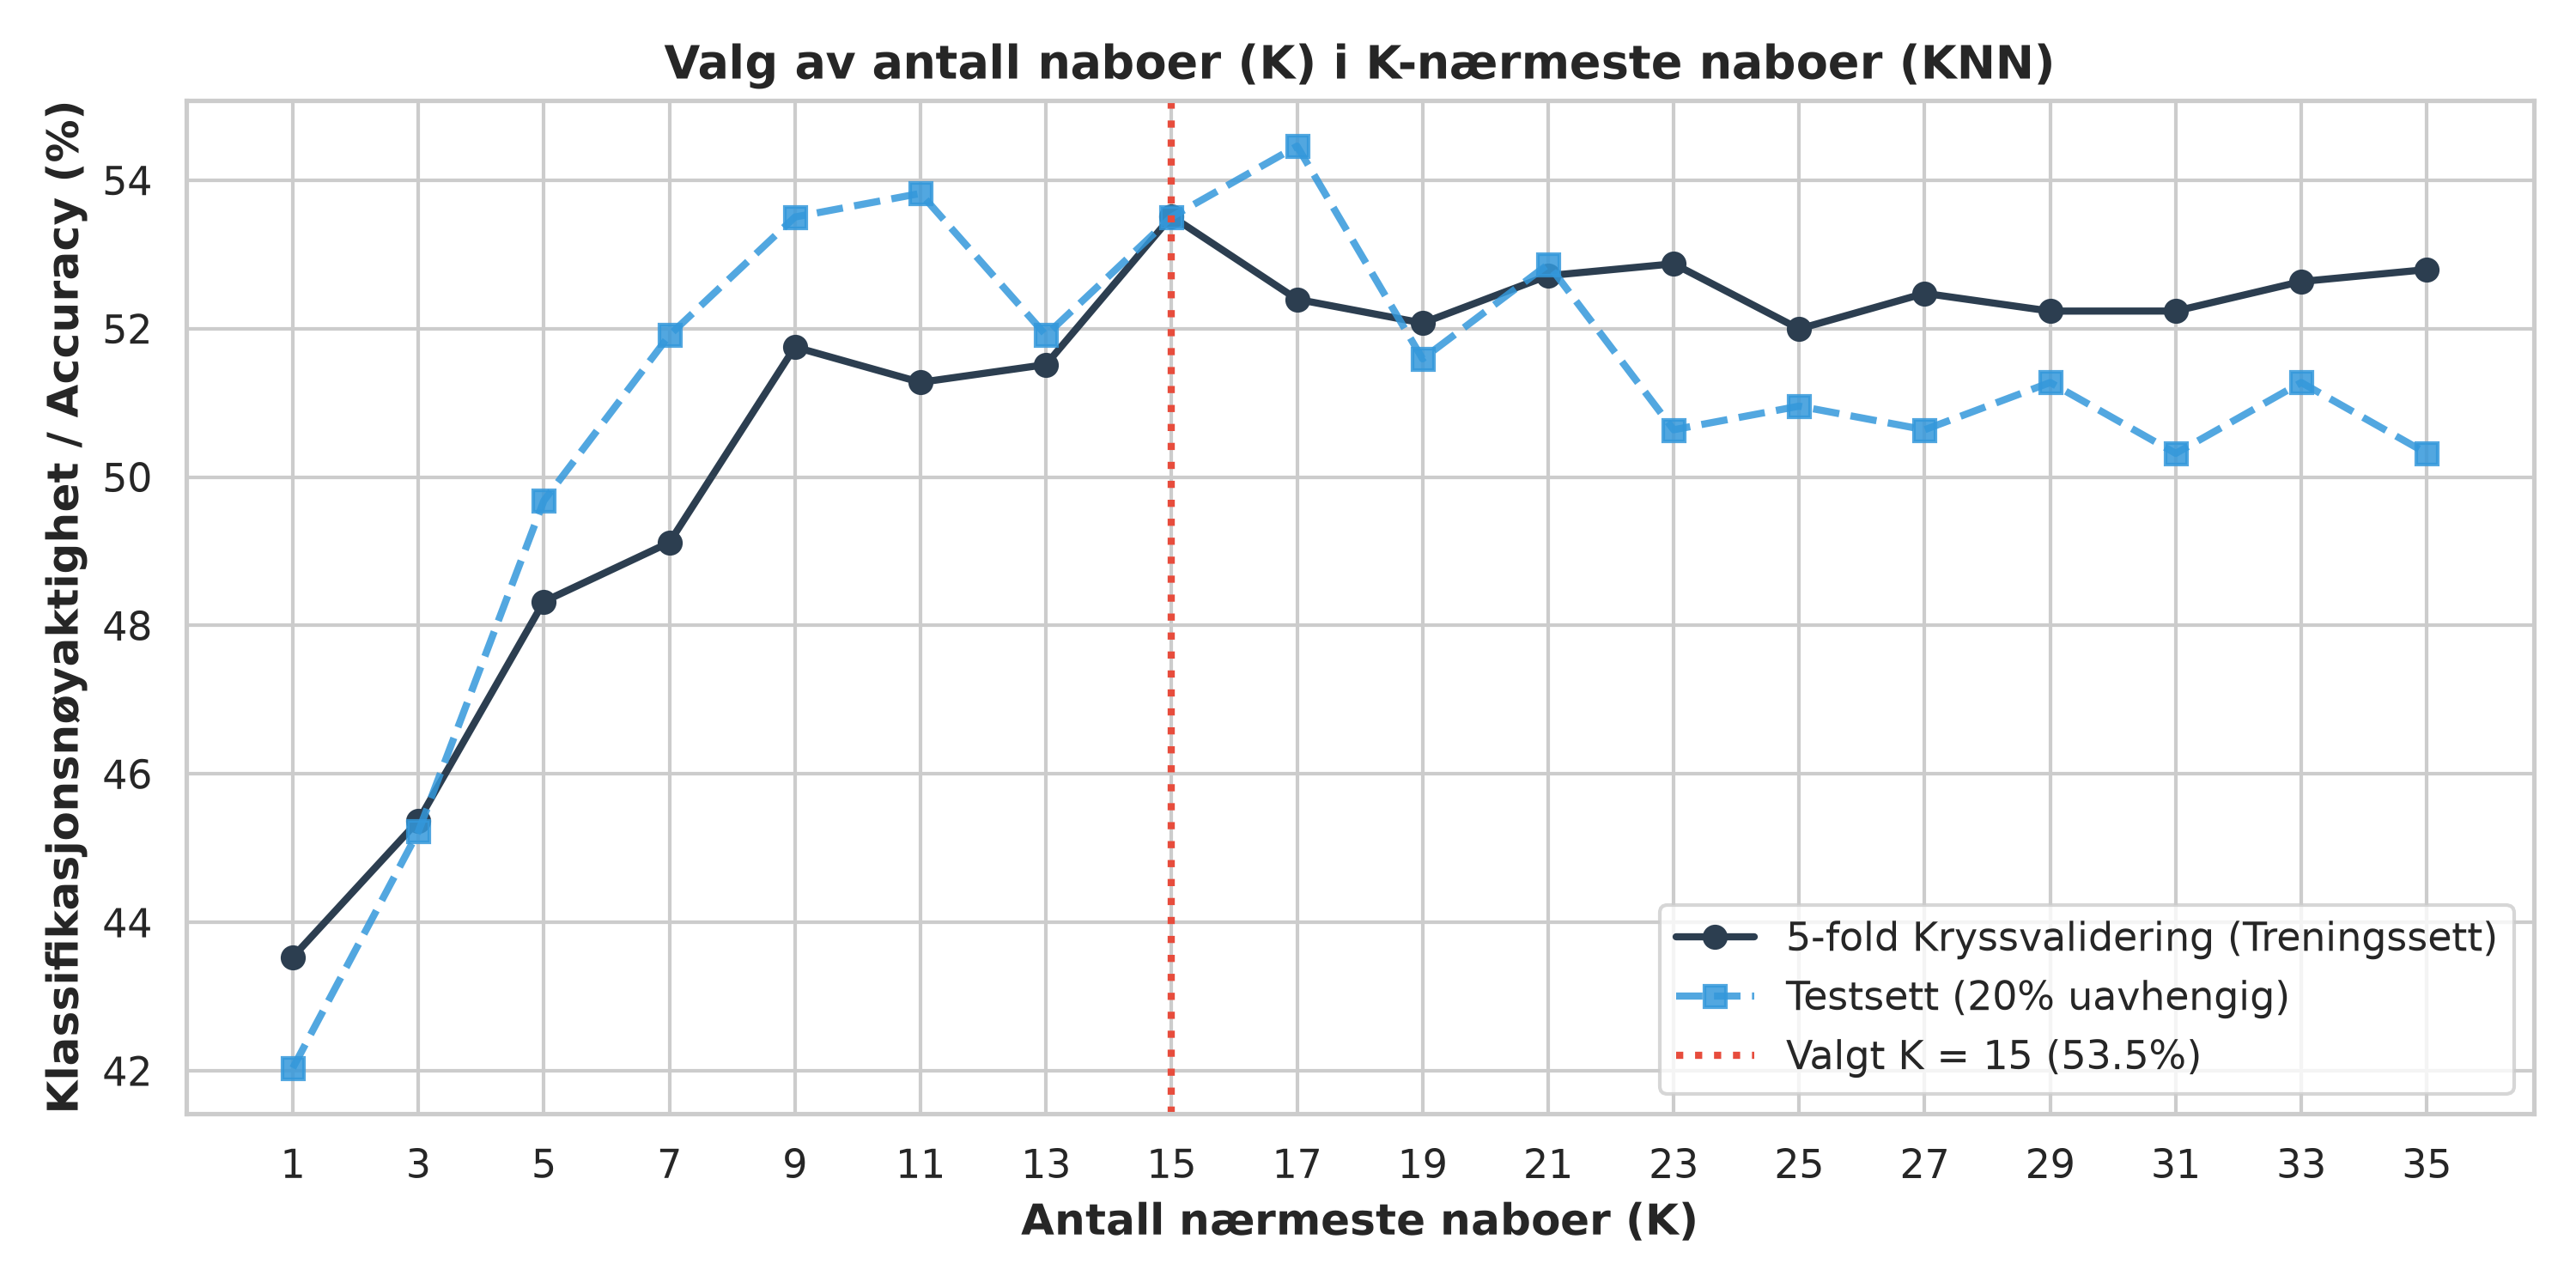
\includegraphics[width=0.88\linewidth]{figurer/7_knn_k_selection.png}
    \caption{Valg av antall naboer $K$ i KNN via 5-fold kryssvalidering på treningssettet ($n = 1252$) sammenlignet med nøyaktighet på testsettet ($n = 314$). Maksimal kryssvalidert nøyaktighet oppnås ved $K = 15$ ($53{,}5\,\%$).}
    \label{fig:knn_k}
\end{figure}

\subsubsection{Evaluering og metodiske begrensninger}
Vi evaluerer metodene med verktøy tilpasset henholdsvis uovervåket og veiledet læring:
\begin{itemize}
\tightlist
\item
  \textbf{Evaluering av klyngeanalyse:} Internt vurderes klyngene med WCSS, silhuett-koeffisienten $s(i) = \frac{b(i) - a(i)}{\max(a(i), b(i))}$ og klyngesentrenes $Z$-score-profiler. Eksternt vurderes klyngene i en kvadratisk ($5 \times 5$) krysstabell mot de fem sjangerfamiliene.
\item
  \textbf{Evaluering av klassifikasjon:} Klassifikasjonsmodellene evalueres på det uavhengige testsettet ($n = 314$) ved hjelp av total treffsikkerhet (\textit{Accuracy}, andel korrekt klassifiserte sanger), en kvadratisk ($5 \times 5$) \textbf{forvirringsmatrise} (\textit{confusion matrix}), samt klassevis \textbf{sensitivitet / recall} ($\frac{\text{TP}}{\text{TP} + \text{FN}}$, hvor stor andel av sangene i en faktisk sjanger modellen fanger opp) og \textbf{presisjon} ($\frac{\text{TP}}{\text{TP} + \text{FP}}$, hvor ofte modellen har rett når den predikerer en gitt sjanger).
\end{itemize}

Det er viktige begrensninger ved både metodene og evalueringsmålene. For det første antar $k$-Means sfæriske klynger av lik utstrekning, mens logistisk regresjon kun kan trekke lineære beslutningsgrenser mellom sjangrene. For det andre er klasseinndelingen i datasettet noe ubalansert (\textit{Pop / Dance} utgjør $434$ sanger, mens \textit{Acoustic / R\&B / Indie} kun utgjør $162$ sanger). I ubalanserte datasett kan total \textit{Accuracy} alene gi et skjevt bilde fordi en modell som favoriserer den største klassen (\textit{Pop / Dance}) oppnår høy total treffsikkerhet på bekostning av lav sensitivitet for mindre klasser. Nettopp derfor supplerer vi \textit{Accuracy} med klassevis sensitivitet (recall), presisjon og hele $5 \times 5$-forvirringsmatrisen. Endelig innebærer generaliseringen av 307 Spotify-undersjangre til fem hovedfamilier at sanger med overlappende stil eller hybride trekk (f.eks.\ pop-rap eller rolige pop-ballader) har en uklar fasit, noe som setter et naturlig tak for hvor høy treffsikkerhet enhver modell basert kun på syv lydmål kan oppnå.

\subsection{Resultater (10 poeng)}\label{resultater-10-poeng}

\begin{enumerate}
\def\labelenumi{\arabic{enumi}.}
\item
  Presenter resultatene på en tydelig og strukturert måte. Dette kan for
  eksempel gjøres ved hjelp av tabeller, grafer eller andre
  visualiseringer som gjør funnene lettere å forstå.
\item
  Tolk resultatene. Tolkningen bør tilpasses regresjons-,
  klassifiserings- eller klyngeanalyse-oppgaven du har valgt.
\item
  Diskuter begrensninger og forbehold som er viktige å ta hensyn til når
  resultatene skal tolkes. Dette kan for eksempel være begrensninger ved
  datasettet, modellene eller evalueringsmetodene.
\item
  (Valgfritt) Se på mulige videre analyser. Beskriv eventuelt
  alternative eller forbedrede metoder som kunne vært brukt for å
  analysere dataene i fremtiden, og hvordan disse potensielt kunne gitt
  ytterligere innsikt.
\end{enumerate}

\subsection{Diskusjon og konklusjon (5 poeng)}\label{diskusjon-og-konklusjon-5-poeng}

Oppsummer de viktigste funnene fra prosjektet deres. Hva fant du ut, og
hvilke var de viktigste innsiktene du fikk gjennom analysen? Fokuser på
de mest relevante resultatene fra modelleringen og analysen.


\newpage
\subsection{Deklarasjon om KI-hjelpemidler (maks 1 side -- teller ikke til de 10 sidene i rapporten)}\label{deklarasjon-om-ki-hjelpemidler-maks-1-side-teller-ikke-til-de-10-sidene-i-rapporten}

Besvar følgende spørsmål:

1.) Har det i utarbeidingen av denne rapporten blitt anvendt KI-baserte
hjelpemidler? Hvis ja, beskriv hvilke verktøy dere brukte (Copilot, NTNU
GPT,\ldots).

2.) Er en eller flere av ideene eller fremgangsmåtene i oppgaven
foreslått av KI? Hvis ja, beskriv her:

3.) Tekst: Har du brukt KI for
\begin{enumerate}
\def\labelenumi{\alph{enumi})}
\tightlist
\item Stavekontroll?
\item Språkvask?
\item Tekstgenerering?
\item Skriveassistanse.
\end{enumerate}

Hvis du svarer ja på minst en av a)-d), spesifiser bruken her:

4.) Kode og algoritmer: Programmeringsassistanse. Er deler av
koden/algoritmene som i) fremtrer direkte i rapporten eller ii) har
blitt anvendt for produksjon av resultater slik som figurer, tabeller
eller tallverdier blitt generert av KI? Hvis ja, spesifiser bruken her:

5.) Bilder og figurer, bildegenerering. Er ett eller flere av
bildene/figurene i rapporten blitt generert av KI? Hvis ja, beskriv
bruken her:

6.) Beskrive alle andre aspekter av arbeidet som KI ble brukt til.
Beskriv her:

7.) Ved innlevering av prosjektet deklarerer vi at vi er kjent med NTNUs
regelverk: Det er ikke tillatt å generere besvarelser eller tekst ved
hjelp av KI og levere den helt eller delvis som eget arbeid. Vi har
derfor redegjort for all anvendelse av KI enten direkte i rapporten,
eller her. Svar her:


\newpage
\subsection{Referanser og kode (teller ikke til de 10 sidene i rapporten)}\label{referanser-og-kode-teller-ikke-til-de-10-sidene-i-rapporten}

Her kan dere legge til alle referanser og kode som dere har brukt for å
generere resultatene i rapporten.


\end{document}
